\documentclass[12pt]{article}
\usepackage[margin=1.0in]{geometry} %page layout
\usepackage[usenames,dvipsnames]{color} %color
\definecolor{light-gray}{gray}{0.95}
\definecolor{darkgreen}{rgb}{0,0.4,0}
\usepackage{graphicx, subfigure} %figures
\usepackage{url, hyperref} %cross-referencing
\usepackage{amsmath, amssymb} %math
\usepackage{listings} %source code
\lstset{breaklines=true,
breakindent=0pt,
prebreak=\mbox{\tiny$\searrow$},
postbreak=\mbox{{\color{blue}\tiny$\rightarrow$}},
numbers=left,
commentstyle=\color{darkgreen},
numberblanklines=false,
frame=single,
captionpos=b,
backgroundcolor=\color{light-gray}}
\usepackage[3D]{movie15} %for movies (needs hyperref)
	\newenvironment{changemargin}[2]
	{
	  	\begin{list}{}
		{
			\setlength{\topsep}{0pt}%
			\setlength{\leftmargin}{#1}%
			\setlength{\rightmargin}{#2}%
			\setlength{\listparindent}{\parindent}%
			\setlength{\itemindent}{\parindent}%
			\setlength{\parsep}{\parskip}%
		}
	  	\item[]
		}
		{\end{list}
	}
\author{Salman Aslam\\Georgia Tech}
\title{RVQ Reconstruction Error Computations}
\author{Salman Aslam\\ Georgia Institute of Technology}
\date{}
\definecolor{darkgreen}{rgb}{0,0.5,0}
\newcommand{\Ntrg}{\big[N_{t=1, m=1} + \lambda \big] + \big[N_{t=1, m=2} + \lambda \big] + \ldots + \big[N_{t=1, m=M} + \lambda \big]}
\newcommand{\jointcnt}{\sum\limits_{n_{trg}=1}^{N_{trg}}I(X_t=x_t, X_{t-1}=x_{t-1})}
\newcommand{\singlecnt}{\sum\limits_{n_{trg}=1}^{N_{trg}}I(X_{t-1}=x_{t-1})}
\newcommand{\singlep}{p(X_{t-1}=x_{t-1})}
\newcommand{\singlepone}{p(X_{t-1}=1)}
\newcommand{\singleptwo}{p(X_{t-1}=2)}
\newcommand{\singlepM}{p(X_{t-1}=M)}
\newcommand{\condp}{p(X_t=x_t | X_{t-1}=x_{t-1})}
\newcommand{\jointp}{p(X_t=x_t, X_{t-1}=x_{t-1})}
\newcommand{\KmeansOuterSum}{\sum\limits_{k=1}^K}
\newcommand{\KmeansInnerSum}{\sum\limits_{{i=1 \atop x_i \in \mathcal{K}_k}}^N}
\newcommand{\KmeansSum}{\KmeansOuterSum \KmeansInnerSum}
\newcommand{\RVQInnerSum}{\sum\limits_{{i=1 \atop g_i \mapsto m_{\tau, s}}}^N}
\newcommand{\RVQOuterSum}{\sum_{s=1}^S}
\newcommand{\RVQsum}{\KmeansOuterSum \sum\limits_{{i=1 \atop g_i \in \mathcal{K}_k}}^N}
\newcommand{\KmeansInner}{{(x_i - \mu_k)}^2}
\newcommand{\RVQinner}{            {(x_i  - \hat{\mu}^{(k)})}^2}
\newcommand{\RVQinneralternate}{{(g_i - m_\tau^{(k)})}^2}
\newcommand{\RVQinneralternatealternate}{{(g_i - m_{\tau, s})}^2}
\newcommand{\KmeansError}{\KmeansSum \KmeansInner}
\newcommand{\RVQerror}     {\KmeansSum \RVQinner}
\newcommand{\RVQerroralternate}{\RVQsum \RVQinneralternate}
\newcommand{\RVQunit}{x_i -\bigg(\sum_{t=1}^Tm^{(k)}_t\bigg)}
\newcommand{\RVQequivalentCodevector}{\sum_{t=1 }^Tm^{(k)}_t}
\newcommand{\RVQequivalentCodevectorBroken}{\sum_{t=1 \atop t \neq \tau}^Tm^{(k)}_t+ m^{(k)}_\tau}
\newcommand{\RVQmultipleKmeans}{x_i -\bigg(\RVQequivalentCodevectorBroken\bigg)}
\newcommand{\RVQmultipleKmeansone}{x_i -\sum_{t=2}^Tm^{(k)}_t+ m^{(k)}_1\bigg)}
\newcommand{\RVQmultipleKmeansonealternate}{\bigg(x_i -\sum_{t=1 \atop t \neq \tau}^Tm^{(k)}_t\bigg) - m^{(k)}_\tau}
\newcommand{\RVQmultipleKmeanstwo}{x_i -\bigg(\sum_{t=1 \atop t \neq 2}^Tm^{(k)}_t+ m^{(k)}_2\bigg)}
\newcommand{\RVQmultipleKmeansT}{x_i -\bigg(\sum_{t=1}^{T-1}m^{(k)}_t+ m^{(k)}_2\bigg)}
\newcommand{\EucMatrix}
{
\left[
\begin{array}{lll}
r_{11} & r_{12} & t_x \\ 
r_{21} & r_{22} & t_y \\ 
0 & 0 & 1 \\ 
\end{array}
\right]
}	

\newcommand{\SimMatrix}
{
\left[
\begin{array}{lll}
sr_{11} & sr_{12} & t_x \\ 
sr_{21} & sr_{22} & t_y \\
0 & 0 & 1 \\ 
\end{array}
\right]
}

\newcommand{\AffMatrix}
{
\left[
\begin{array}{lll}
a &b & t_x \\ 
c & d & t_y \\
0 & 0 & 1 \\
\end{array}
\right]
}

\newcommand{\ProjMatrix}
{
\left[
\begin{array}{lll}
h_{11} & h_{12} & h_{13} \\ 
h_{21} & h_{22} & h_{23} \\ 
h_{31} & h_{32} & h_{33} \\ 
\end{array}
\right]
}

\newcommand{\RotMatrixTheta}
{
\left[
\begin{array}{rr}
\cos(\theta) & -\sin(\theta) \\ 
\sin(\theta) & \cos(\theta) \\ 
\end{array}
\right]
}

\newcommand{\RotMatrixPhi}
{
\left[
\begin{array}{rr}
\cos(\phi) & -\sin(\phi) \\ 
\sin(\phi) & \cos(\phi) \\ 
\end{array}
\right]
}

\newcommand{\RotMatrixminusPhi}
{
\left[
\begin{array}{rr}
\cos(-\phi) & -\sin(-\phi) \\ 
\sin(-\phi) & \cos(-\phi) \\ 
\end{array}
\right]
}


\newcommand{\EigenvalueMatrix}
{
\left[
\begin{array}{cc}
\lambda_1 & 0\\
0 & \lambda_2
\end{array}
\right]
}

\newcommand{\bigMatrix}
{
s \left[
\begin{array}{cc}
 (r)(a) + b &  (r)(d) - c \\
 (r)(c) - d &  (r)(b) + a
\end{array}
\right]
}


\newcommand{\bigMatrixTwo}
{
\left[
\begin{array}{cc}
(\lambda_2) p + (\lambda_1) q & (\lambda_2) s  - (\lambda_1) r \\
(\lambda_2) r  - (\lambda_1) s & (\lambda_2) q + (\lambda_1) p
\end{array}
\right]
}
\newcommand{\dr}{(\mathbf{x}_i-\boldsymbol\mu_k)^T(\mathbf{x}_i-\boldsymbol\mu_k) + \lambda({Q_{\textrm{max}}-Q_i})}

\begin{document}
\maketitle
\rule[0pt]{\textwidth}{1pt}
\tableofcontents
\rule[0pt]{\textwidth}{1pt}


%===================================
\section{Introduction}
%===================================
In this report, we look at a simple training set, $S_{trg}=\{1,2,3,4,5,6,7\}$ and design RVQ encoder and decoder codebooks for different number of code-books per stage, $m=\{2,3,4,5,6,7,8\}$.  Our goal is to understand when encoder and decoder codebooks differ, and how stagewise computations for reconstruction rms error are carried out.


%===================================
\section{Experiments}
%===================================
%We start with some trivial scalar examples where the training and test sets are the same.  We then move to the other extreme end of the spectrum using random data in high dimensional spaces with several observations and where the training and test sets have the same distributions but have different data.  After these experiments, we will get to tracking examples and use the likelihood formulation we have developed for RVQ.

Table~\ref{table:encoder} gives the encoder codebooks while Table~\ref{table:decoder} gives the decoder codebooks for our training set.  Notice that all codebooks are the same except for the 3x2 case.  For reference, the output of gen.exe for the 2x3 case is given in Appendix~\ref{gen_stat}.

\begin{table}
\centering
\subtable[3x{\color{red}\textbf 2}]{\begin{tabular}{|c|c|}\hline 
2.5  & 6\\
-1  & 1\\
-0.5  & 0.5\\\hline
\end{tabular}}\hspace{0.2in}
\subtable[2x{\color{red}\textbf 3}]{\begin{tabular}{|c|c|c|}\hline
1.5 & 6.5 & 4\\
-1 & 0.667 & -0.5\\\hline
\end{tabular}}\hspace{0.2in}
\subtable[2x{\color{red}\textbf 4}]{\begin{tabular}{|c|c|c|c|}\hline
1 & 6.5 & 4 & 2\\
-1 & 1 & -0.5 & 0.5\\\hline
\end{tabular}}\hspace{0.2in}
\subtable[2x{\color{red}\textbf 5}]{\begin{tabular}{|c|c|c|c|c|}\hline
1 & 6.5 & 4.5 & 2 & 3\\
-0.5 & 0.5 & 0 & 0 &0\\\hline
\end{tabular}}\hspace{0.2in}
\subtable[2x{\color{red}\textbf 6}]{\begin{tabular}{|c|c|c|c|c|c|}\hline
1 & 6.5 & 4 & 2 & 3 &5\\
-0.5 & 0.5 & 0 & 0 &0 &0\\\hline
\end{tabular}}\hspace{0.2in}
\subtable[1x{\color{red}\textbf 7}]{\begin{tabular}{|c|c|c|c|c|c|c|}\hline
1 & 7 & 4 & 2 & 3 &5 &6\\\hline
\end{tabular}}
\hspace{0.2in}
\subtable[1x{\color{red}\textbf 8}]{\begin{tabular}{|c|c|c|c|c|c|c|c|}\hline
1 & 7 & 4 & 2 & 3 &5 &6&0\\\hline
\end{tabular}}
\caption{RVQ \emph{encoder} codebooks with increasing code-vectors per stage, $m$ = {\color{red}\textbf {2, 3, 4, 5, 6, 7, 8}}.  As $m$ goes up for a given training set, the number of stages $q$ falls.}
\label{table:encoder}
\end{table}



\begin{table}
\centering
\subtable[3x{\color{red}\textbf 2}]{\begin{tabular}{|c|}\hline
same as encoder\\codebook\\\hline
\end{tabular}}\hspace{0.2in}
\subtable[2x{\color{red}\textbf 3}]{\begin{tabular}{|c|c|c|}\hline
-1 & 6 & 4\\
-1 & 1 & 0\\\hline
\end{tabular}}\hspace{0.2in}
\subtable[3x{\color{red}\textbf 4}]{\begin{tabular}{|c|}\hline
same as encoder\\codebook\\\hline
\end{tabular}}\hspace{0.2in}
\subtable[3x{\color{red}\textbf 5}]{\begin{tabular}{|c|}\hline
same as encoder\\codebook\\\hline
\end{tabular}}\hspace{0.2in}
\subtable[3x{\color{red}\textbf 6}]{\begin{tabular}{|c|}\hline
same as encoder\\codebook\\\hline
\end{tabular}}\hspace{0.2in}
\subtable[3x{\color{red}\textbf 7}]{\begin{tabular}{|c|}\hline
same as encoder\\codebook\\\hline
\end{tabular}}\hspace{0.2in}
\subtable[3x{\color{red}\textbf 8}]{\begin{tabular}{|c|}\hline
same as encoder\\codebook\\\hline
\end{tabular}}
\caption{RVQ \emph{decoder} codebooks with increasing code-vectors per stage, $m$ = {\color{red}\textbf {2, 3, 4, 5, 6, 7, 8}}.}
\label{table:decoder}
\end{table}

For the 2x3 encoder codebook, the reconstruction rms errors, $e_1$ and $e_2$ after stages 1 and 2 respectively are,

\begin{equation}
\begin{array}{lllll}
e_1 &= \sqrt \frac{4(0.5^2) + 3(1^2)}{7} &= \sqrt\frac{3}{7} &= 0.6547 \\
e_2 &= \sqrt \frac{2(0.1667^2) + 0.5^2 + 0.3333^2}{7} &= \sqrt\frac{0.4167}{7} &= 0.2440 
\end{array}
\end{equation}

The actual rms errors as reported by gen.exe as given in Appendix~\ref{gen_stat} and plotted in Figure~\ref{fig:RVQ_8x3_trg_1_to_7} are 0.6547 and 0.1543 respectively.

\begin{table}[t]
\centering
\subtable[3x{\color{red}\textbf 2}]{\begin{tabular}{|c||c|c|c|c|c|c|c|}\hline 
\textbf{Test point} $\rightarrow$& \textbf{1}    & \textbf{2}  &   \textbf{3}    &      \textbf{4}  &   \textbf{5} &   \textbf{6} &   \textbf{7}\\\hline
\textbf{recon. error after stage 1} $\rightarrow$& 0.5    & 0.5  &   1    &      0  &   1  &   0.5 &    0.5\\
\textbf{recon. error after stage 2} $\rightarrow$& 0  &   0.1667    &      0  &   0.5  &   0.3333    &      0  &   0.1667\\\hline
\end{tabular}}
\caption{RVQ reconstruction error using 2x3 \emph{encoder} codebook.}
\label{table:encoder_recon}
\end{table}

								\begin{figure}
								\centering
								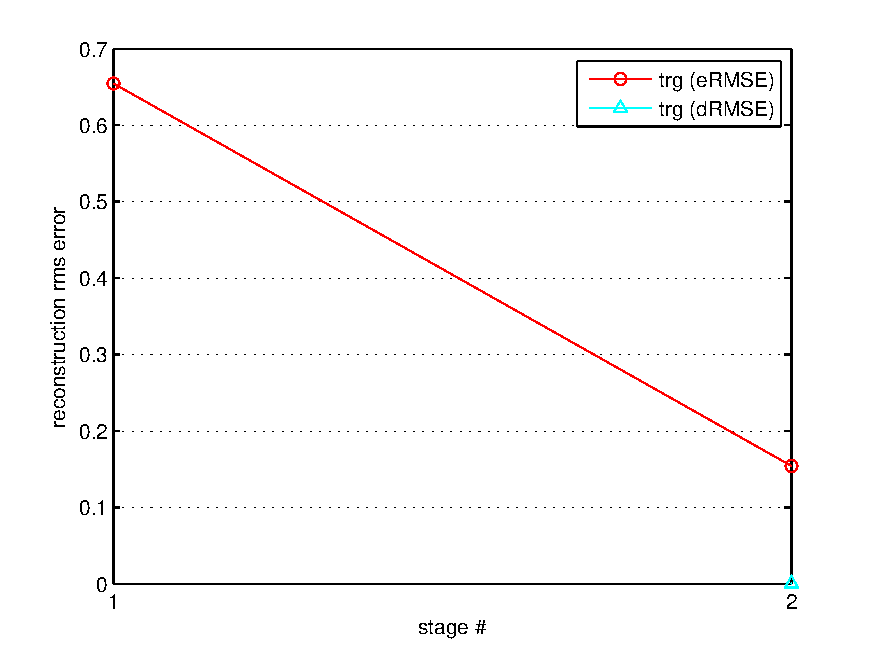
\includegraphics[width=0.75\textwidth]{figs/RVQ_8x3_trg_1_to_7.pdf}
								\caption{eRMSE=\{0.6547, 0.1543\} for stages 1 and 2, and dRMSE=\{0\} for stage 2, as reported by gen.exe for 2x3 RVQ.  The training set is $S_{trg}=\{1,2,3,4,5,6,7\}$.}
								\label{fig:RVQ_8x3_trg_1_to_7}
								\end{figure}


%===================================
\section{Conclusions}
%===================================
For the first stage, we are able to reconcile our rms computations with those reported by gen.exe.  However, for the second stage, we are unable to reconcile the computations.  We need to investigate this further.

\clearpage
\newpage
\appendix
%===================================
\section{gen\_stat file output for 2x3 RVQ}
\label{gen_stat}
%===================================
\scriptsize
\begin{verbatim}
RVQ__training_gen8.exe 7_posEg_1x1.raw 7_codebook.ecbk 7_codebook.dcbk 4 -S1000 -i0.0005 -j0.0005 
getts:Initial Training Cummulative Distortion = 1.3235e+006
Seeding Stage #1
prime_cbks:GLA Codevec Cummulative Distortion = 5.4600e+002:2:
prime_cbks:GLA Codevec Cummulative Distortion = 1.1400e+002:3:3.789474
prime_cbks:GLA Encoder Cummulative Distortion = 2.4000e+001:4:
prime_cbks:GLA Encoder Cummulative Distortion = 1.8000e+001:4:0.333333
prime_cbks:GLA Encoder Cummulative Distortion = 1.8000e+001:4:0.000000
encode:New Encoder Cummulative Distortion = 1.8000e+001:+1323507.000000
Encoder:RelChg=+73528.1667:eSNR=48.66:eRMSE=  0.6547:sws=0
Number Still Growing = 6
  1->    2     2     3     0 
Amoratized Fixed-Rate Coding =  0.2642 bits per sample
Number-of-Stages Overhead    =  0.0000 bits per sample
Average Number-of-Stages     =  1.0000
Seeding Stage #2
prime_cbks:GLA Codevec Cummulative Distortion = 5.4000e+001:2:
prime_cbks:GLA Codevec Cummulative Distortion = 6.0000e+000:3:8.000000
prime_cbks:GLA Encoder Cummulative Distortion = 3.0000e+000:4:
prime_cbks:GLA Encoder Cummulative Distortion = 1.0000e+000:4:2.000000
prime_cbks:GLA Encoder Cummulative Distortion = 1.0000e+000:4:0.000000
encode:New Encoder Cummulative Distortion = 1.0000e+000:+17.000000
Encoder:RelChg=+17.0000:eSNR=61.22:eRMSE=  0.1543:sws=0
decode:Old Decoder Cummulative Distortion = 1.0000e+000
decode:New Decoder Cummulative Distortion = 6.1111e-001:0.636364
decode:New Decoder Cummulative Distortion = 3.6814e-001:0.659991
decode:New Decoder Cummulative Distortion = 2.8774e-001:0.279417
decode:New Decoder Cummulative Distortion = 2.3707e-001:0.213751
decode:New Decoder Cummulative Distortion = 1.9705e-001:0.203097
decode:New Decoder Cummulative Distortion = 1.6402e-001:0.201386
decode:New Decoder Cummulative Distortion = 1.3655e-001:0.201112
decode:New Decoder Cummulative Distortion = 1.1369e-001:0.201068
decode:New Decoder Cummulative Distortion = 9.4662e-002:0.201061
decode:New Decoder Cummulative Distortion = 7.8815e-002:0.201060
decode:New Decoder Cummulative Distortion = 6.5621e-002:0.201059
decode:New Decoder Cummulative Distortion = 5.4636e-002:0.201059
decode:New Decoder Cummulative Distortion = 4.5490e-002:0.201059
decode:New Decoder Cummulative Distortion = 3.7875e-002:0.201059
decode:New Decoder Cummulative Distortion = 3.1535e-002:0.201059
decode:New Decoder Cummulative Distortion = 2.6256e-002:0.201059
decode:New Decoder Cummulative Distortion = 2.1860e-002:0.201059
decode:New Decoder Cummulative Distortion = 1.8201e-002:0.201059
decode:New Decoder Cummulative Distortion = 1.5154e-002:0.201059
decode:New Decoder Cummulative Distortion = 1.2617e-002:0.201059
decode:New Decoder Cummulative Distortion = 1.0505e-002:0.201059
decode:New Decoder Cummulative Distortion = 8.7465e-003:0.201059
decode:New Decoder Cummulative Distortion = 7.2823e-003:0.201059
decode:New Decoder Cummulative Distortion = 6.0633e-003:0.201059
decode:New Decoder Cummulative Distortion = 5.0483e-003:0.201059
decode:New Decoder Cummulative Distortion = 4.2032e-003:0.201059
decode:New Decoder Cummulative Distortion = 3.4996e-003:0.201059
decode:New Decoder Cummulative Distortion = 2.9137e-003:0.201059
decode:New Decoder Cummulative Distortion = 2.4260e-003:0.201059
decode:New Decoder Cummulative Distortion = 2.0199e-003:0.201059
decode:New Decoder Cummulative Distortion = 1.6817e-003:0.201059
decode:New Decoder Cummulative Distortion = 1.4002e-003:0.201059
decode:New Decoder Cummulative Distortion = 1.1658e-003:0.201059
decode:New Decoder Cummulative Distortion = 9.7065e-004:0.201059
decode:New Decoder Cummulative Distortion = 8.0816e-004:0.201059
decode:New Decoder Cummulative Distortion = 6.7287e-004:0.201059
decode:New Decoder Cummulative Distortion = 5.6023e-004:0.201059
decode:New Decoder Cummulative Distortion = 4.6645e-004:0.201059
decode:New Decoder Cummulative Distortion = 3.8836e-004:0.201059
decode:New Decoder Cummulative Distortion = 3.2335e-004:0.201059
decode:New Decoder Cummulative Distortion = 2.6922e-004:0.201059
decode:New Decoder Cummulative Distortion = 2.2415e-004:0.201059
decode:New Decoder Cummulative Distortion = 1.8663e-004:0.201059
decode:New Decoder Cummulative Distortion = 1.5539e-004:0.201059
decode:New Decoder Cummulative Distortion = 1.2938e-004:0.201059
decode:New Decoder Cummulative Distortion = 1.0772e-004:0.201059
decode:New Decoder Cummulative Distortion = 8.9686e-005:0.201059
decode:New Decoder Cummulative Distortion = 7.4672e-005:0.201059
decode:New Decoder Cummulative Distortion = 6.2172e-005:0.201059
decode:New Decoder Cummulative Distortion = 5.1764e-005:0.201059
decode:New Decoder Cummulative Distortion = 4.3099e-005:0.201059
decode:New Decoder Cummulative Distortion = 3.5884e-005:0.201059
decode:New Decoder Cummulative Distortion = 2.9877e-005:0.201059
decode:New Decoder Cummulative Distortion = 2.4876e-005:0.201059
decode:New Decoder Cummulative Distortion = 2.0711e-005:0.201059
decode:New Decoder Cummulative Distortion = 1.7244e-005:0.201059
decode:New Decoder Cummulative Distortion = 1.4358e-005:0.201059
decode:New Decoder Cummulative Distortion = 1.1954e-005:0.201059
decode:New Decoder Cummulative Distortion = 9.9529e-006:0.201059
decode:New Decoder Cummulative Distortion = 8.2868e-006:0.201059
decode:New Decoder Cummulative Distortion = 6.8996e-006:0.201059
decode:New Decoder Cummulative Distortion = 5.7446e-006:0.201059
decode:New Decoder Cummulative Distortion = 4.7829e-006:0.201059
decode:New Decoder Cummulative Distortion = 3.9822e-006:0.201059
decode:New Decoder Cummulative Distortion = 3.3156e-006:0.201059
decode:New Decoder Cummulative Distortion = 2.7606e-006:0.201059
decode:New Decoder Cummulative Distortion = 2.2985e-006:0.201059
decode:New Decoder Cummulative Distortion = 1.9137e-006:0.201059
decode:New Decoder Cummulative Distortion = 1.5933e-006:0.201059
decode:New Decoder Cummulative Distortion = 1.3266e-006:0.201059
decode:New Decoder Cummulative Distortion = 1.1045e-006:0.201059
decode:New Decoder Cummulative Distortion = 9.1963e-007:0.201059

Decoder Cummulative Distortion is Less Than 0.000001
Decoder:RelChg=+1087393.6544:dSNR=121.58:dRMSE=  0.0001
Number Still Growing = 3
  1->    2     2     3     0 
  2->    1     3     2     0 
Amoratized Fixed-Rate Coding =  0.4906 bits per sample
Number-of-Stages Overhead    =  0.1667 bits per sample
Average Number-of-Stages     =  1.8571

TERMINATING PROGRAM
\end{verbatim}
\normalsize


\clearpage
\newpage
\normalsize
\bibliographystyle{ieee}
\bibliography{MyCitations}
\end{document}